\placeholder{[Alice] So did bug 7 never cause the program to fail, or
did it not only not cause the program to fail, but also managed to
produce the correct output?  If it's the latter, we should explicitly
state that, seeing the amount of detail we went into in the last
section to describe how a run is judged to have ``failed.''}

This section describes the results of applying the algorithm discussed
in \Autoref{sec:algorithm} to the experiment described in
\Autoref{sec:experiments:setup}.  We briefly summarize the results.
The algorithm identified a cause that would be useful to a programmer
examining these results for 7 of the 9 bugs.  For the 2 other bugs,
one of the bugs (bug \#7) occurred in our experiment but never caused
the program to fail; the other missing bug (bug \#8) was never
triggered at all.  For 5 of the 7 bugs that led to program failures,
the causes of the bugs were ranked very high in the initial results.  The
remaining 2 bugs had causes that were ranked very near the top once
we removed the other 5 bugs we ``found'' with our tool from the
experiment.  A surprise was that we found a bug \#10; the results
showed us a previously undiscovered bug in \moss.

We performed 31,996 random runs of \moss.  Of these, 123 runs were
discarded because they produced no report (see
\Autoref{sec:experiments:setup}), giving us 31,873 runs to work with.

For this experiment we enabled all three instrumentation strategies
described in \Autoref{sec:background}:

\begin{description}
\item[branches:] 2,085 instrumentation sites.  Each site has two
  counters and yields two predicates, for 4,170 branch predicates over
  all.

\item[returns:] 494 instrumentation sites.  Each site has three
  counters and yields six predicates, for 2,964 return predicates over
  all.

\item[scalar-pairs:] 32,644 instrumentation sites.  Each site has
  three counters and yields six predicates, for 195,864 scalar-pair
  predicates over all.
\end{description}

\placeholder{[Alice] Where are we going to mention compound
  predicates?  This affects our footnote below: we are not actually
  recording 200,000 predicates; we are only recording 103584
  predicates, the rest are synthesized from them.}

Thus, the input to our analysis is 31,873 feedback reports, each of which records the
status of over 200,000 predicates.\footnote{The reader may wonder
whether it is practical to actually generate a report on 200,000
predicates on a client machine and then upload it to a central server
for analysis.  The answer is definitely yes.  These reports are mostly
zeroes and so compress extremely well, resulting in uploaded files in
the range of 10-50K.}  The sampling rate for all runs in this
experiment was \nicefrac{1}{1}; i.e., we sampled every predicate every time it was
reached.  We used a separate downsampling program to generate sparser
samples from this full data; thus, we were able to use the same set of
runs to test the effect of different sampling rates on the results.

The time to run our algorithm on all the runs is about seven minutes on
a fast machine.

Step (1) of our analysis algorithm eliminates almost all of the
predicates.  For example, at \nicefrac{1}{100} sampling, the numbers
of predicates with a positive
$\increase(\ldots)$ score are
\placeholder{[Alice] Hmm, I have different numbers here: 38 branch
  predicates, 28 return predicates, and 8243 scalar-pairs.}

\begin{itemize}
\item 51 branch predicates;

\item 16 return predicates;

\item 8,672 scalar-pair predicates.
\end{itemize}
\placeholder{[Alice] Is this percentage ``in general,'' or ``in this
  case''?  We should state that.}
%About 99\% of all predicates in the the branch and returns
%instrumentation strategies are eliminated by step (1) of our
%algorithm.  About 96\% of the predicates in the scalar-pairs strategy are
%eliminated, but clearly this list is too long to process by hand,
In this case, Step (1) of our analysis algorithm eliminates about 99\% of
all branch and return predicates, and about 96\% of the scalar-pairs
predicates.  But clearly this list is too long to process by hand,
even if we only look at the highly-ranked predicates.  We noticed that
the cause of the redundancy is that many closely related predicates
are reported for the
same line number.  Often there is a logically strongest predicate that can be
selected; for example, if the system observes that $\tt x \leq y$ and $\tt x < y$
are both correlated with failure, the predicate $\tt x \leq y$ is clearly redundant.
For our experiment, we simply reported only one predicate per line,
and then browsed the entire list of other predicates on that line if it
appeared interesting.  Retaining one predicate per line gave us a list
of 186 lines to examine (i.e., only 186 distinct lines in the program had
predicates that were correlated with failure).

\subsection{The Bugs}

Because the branches instrumentation and the returns instrumentation
yield high quality predicates, we began by examining those two lists.  We expect this is
what a programmer or QA engineer examining these results would do as well.

\placeholder{[Alice] Suggestion: change the figure to a tabel and put
  ``Increase'', ``Crash'', and ``Context'' in the column headers.}

\begin{figure}
\centering
\begin{small}
  \begin{BVerbatim}[gobble=4]
    0.94 Inc, 1.00 Cr, 0.06 Co, process_file_pass2, line 5523
    0.80 Inc, 1.00 Cr, 0.20 Co, handle_options, line 5742
    0.80 Inc, 1.00 Cr, 0.20 Co, string2lang, line 4366
    0.78 Inc, 1.00 Cr, 0.22 Co, handle_options, line 5789
  \end{BVerbatim}
\end{small}

\caption{The top four entries from the branches report.}
\label{fig-report}
\end{figure}

\placeholder{[Alice] Are these results obtained from the 1/100
  downsampled data?
  We switch to talking about results from the full data somewhere in
  the middle of this section, but we never said what the dataset was
  that we used before then.}

The branches report has 4 predicates with a 1.0 crash rating, shown in
Figure~\ref{fig-report}.  Each line of the report lists the increase,
crash, and context scores of a predicate, as well as the function name
and line number where it occurs.  We have dropped some fields of the
report (such as the text of the predicate itself and the number of
failing and successful runs in which the predicate is observed) to
avoid cluttering the figure.

The first predicate listed does not immediately suggest what the cause
of failure might be. By looking at the failure log, we see that this predicate
is highly correlated with a subset of the runs in which bug \#6 is
triggered; an engineer with a deep understanding of how \moss\ works
might be able to figure out the bug from this predicate alone.
\placeholder{Need to confirm with Mayur that in fact this predicate is bug \#6.}
The next three predicates are obvious ``hits''. The second predicate
says that when comment matching is turned on, the program is
guaranteed to fail; this is bug \#1, and the predicate points directly
to the fact that something is wrong in the comment matching code.
\placeholder{[Alice] Moved to footnote.}
\footnote{Recall that bug \#1 is non-deterministic; why then is the crash score 1.0?
The discrepancy is the result of sampling error.  In the full data set
(with \nicefrac{1}{1} sampling) the crash measure for this predicate is indeed
only .88.}
The
next predicate marks the test for whether \moss\ is analyzing Lisp
programs; the crash score of 1.0 tells us that whenever a Lisp program is
processed, \moss\ crashes.  The last predicate in
Figure~\ref{fig-report} is a much more obvious cause of
bug \#6; it reveals that whenever the amount of memory to use is set
via a command line option, the program will crash.\footnote{The full data set shows that bug \#6 is non-deterministic with respect to this predicate, so once again the certainty that the program will crash is the result of sampling error.}  All three of these predicates illustrate the potential of our method to
help pinpoint the root cause of a crash rather than just where the crash
happened.  Each of these predicates immediately suggests
what test case to try to reproduce the bug.

\placeholder{[Alice] I think we need to put more details about the
  predicates into Figure 1.  As it is, it doesn't say anything that
  Alex wrote about in the above paragraph.  Maybe we should show the
  exact line of the program text along side each predicate?}

The 9th listed cause in the branches report says that whenever the
user supplies the command line option to write a database, the chance
of failure jumps to 62\% (bug \#2), and the fourteenth ranked cause
says that whenever a database is read the chance of failure is 55\%
(bug \#3).  All the other causes between the 5th and 21st in the branches report are predicates that also implicate one of bugs 1, 2, 3, 5, or 6.  Below
the 22nd listed cause the $\increase(\ldots)$ score for the predicates is
only 1\%; we did not examine these predicates.

The returns report is also quite interesting.  Recall that this
instrumentation scheme samples the return values of functions (whether
they are negative, positive, or zero).  The first two entries in this
report are the results of string comparisons that point directly to bug
\#5.  The third entry is the {\tt open} call in the function that writes
a database; the predicate shows that when this function returns {\tt NULL},
the program is guaranteed to crash (i.e., 1.0 crash score).  This is the
cause of bug \#2.

The fourth entry of the full data (not the \nicefrac{1}{100} downsampled data)
returns report is very interesting.  This predicate shows that one of
the file read operations in the function that loads a database can
fail, and when it does \moss\ itself fails with probability 0.64.
It turns out that \moss\ was written assuming that the databases it
loaded would never be corrupt,
\placeholder{[Alice] I can't parse this next sentence.}
because it does no checking to ensure
that the file reads that load databases succeed.  This is a previously
unknown bug in \moss.  It is a bit surprising that it was detected,
because a run is only labeled a failure in our experiment if the
reference \moss\ and the buggy \moss\ differ in their outcome, and
this bug is present in both.  Thus, this bug could only be detected
when another one of the introduced bugs was also triggered in the same
run and caused the buggy version of \moss\ to fail in a different way.
This explains the very low $\increase(\ldots)$ score for this
predicate (the chance of failure only increases by 11\% when this bug
occurs) and why it was not observed in the \nicefrac{1}{100}
downsampled data.\footnote{With enough runs it would be observed at
  any sampling rate, but the anomaly that the reference and buggy
  versions of \moss\ share this bug means that, at the
  \nicefrac{1}{100} sampling rate, many more runs are likely needed
  than what we had for this experiment.}

Bugs \#4 and \#9 have no causes in either the branches or the returns
reports, as they are not correlated with any branch nor correlated
with the result of any function call.  In the scalar-pairs report they
are ranked 26th (for bug \#4) and 52nd (for bug \#9).  In both cases
all of the predicates reported on the line reported were obvious
indicators for the bug, so it did not matter in this case which
predicate was selected as the representative for the report.  The
predicates ranked higher than these two are either more obscure,
but more deterministic, indicators for bug \#4 or for one of the other five observed bugs.
Given the emphasis on determinism in our ranking function, bug \#9 could not be listed
higher, as it is the most non-deterministic bug in our data set with a
$\crash(\ldots)$ score of 0.72.

\placeholder{[Alice] Again, were the results stated above from the
  1/100 sampled data or the 1/1 sampled data?}

Finally, we compared the reports generated from \nicefrac{1}{100} sampled data
with the reports generated from \nicefrac{1}{1} sampled data.  The reports were
similar, but not identical.  In particular the ordering of the
predicates was slightly different and a few predicates with relatively
few observations or a low $\increase(\ldots)$ score, and thus very
sensitive to whether one or two successful or failing runs were
observed or not, appeared on
%one list and not the other.
the 1/1 list but not the 1/100 sampled list.

\placeholder{ We need to comment on the ``big picture'' with our results,
and observe the relative weakness of scalar pairs compared to the other two.
We should also revisit the two bugs that did not cause failure and remind the
reader that part of our goal is to triage bugs, and bugs that don't occur
are triaged out of existence.}

\subsection{Analysis of Predicate Elimination}

Figure \ref{predelim} characterizes the predicates that are eliminated by
the algorithm, namely, predicates $P$ such that $Increase(P) \leq 0$.
A {\it dead} predicate is one that is not observed in any run and hence
deemed unreachable.
An {\it invariant} is a predicate that is observed in some run and, moreover,
is either true every time it is observed or false every time it is observed,
and is therefore presumed to be a program invariant.
An {\it aftermath} is a predicate that is not observed in any successful run but
is observed in some failing run, and is therefore deemed to be a secondary consequence
of a bug.

\begin{figure}[h]
\begin{center}
\begin{tabular}{|l|r|r|r|r|}
\hline
predicate &  \multicolumn{4}{c|}{sampling rate} \\
\cline{2-5}
category  &  1/1 & 1/10 & 1/100 & 1/1000 \\
\hline
\hline
dead      &  92810 & 92810 & 92834 & 95210 \\
\hline
invariant &  56418 & 56614 & 57082 & 57034 \\
\hline
aftermath &  5666  & 5954  & 6534  & 7032 \\
\hline
misc.     &  38762 & 36768 & 36504 & 33023 \\
\hline
\end{tabular}
\caption{Classification of eliminated predicates.}
\label{predelim}
\end{center}
\end{figure}

\subsection{Effect of Sampling on Predicate Selection}

Having discussed the quality of our results, we now turn to the more
quantitative measures.  Specifically, how is the size of the set of
selected predicates affected by the sampling rate and the number of
program trials we include in our dataset?  Figure~\ref{fig-predkept}(a)
shows the effects of sampling and the size of the data on our
algorithm.  For each sampling rate, we start with $3000$ randomly
selected trial runs, and add $3000$ random trials at a time, until we
incorporate all $31873$ runs of our data.  We record the number of
predicates retained at each step.  This process is repeated 10 times,
with 10 different random permutation sequences
of our data. We plot the mean and the confidence interval of one
standard deviation above and below the mean.  When all $31873$ trial
runs are used, we retain $8129$ predicates when the data is not
sampled (i.e. sampling rate is $\nicefrac{1}{1}$), $8807$ at sampling
rate $\nicefrac{1}{10}$, $8309$ at $\nicefrac{1}{100}$, and $8936$ at
$\nicefrac{1}{1000}$.

\begin{figure}
  \centering
  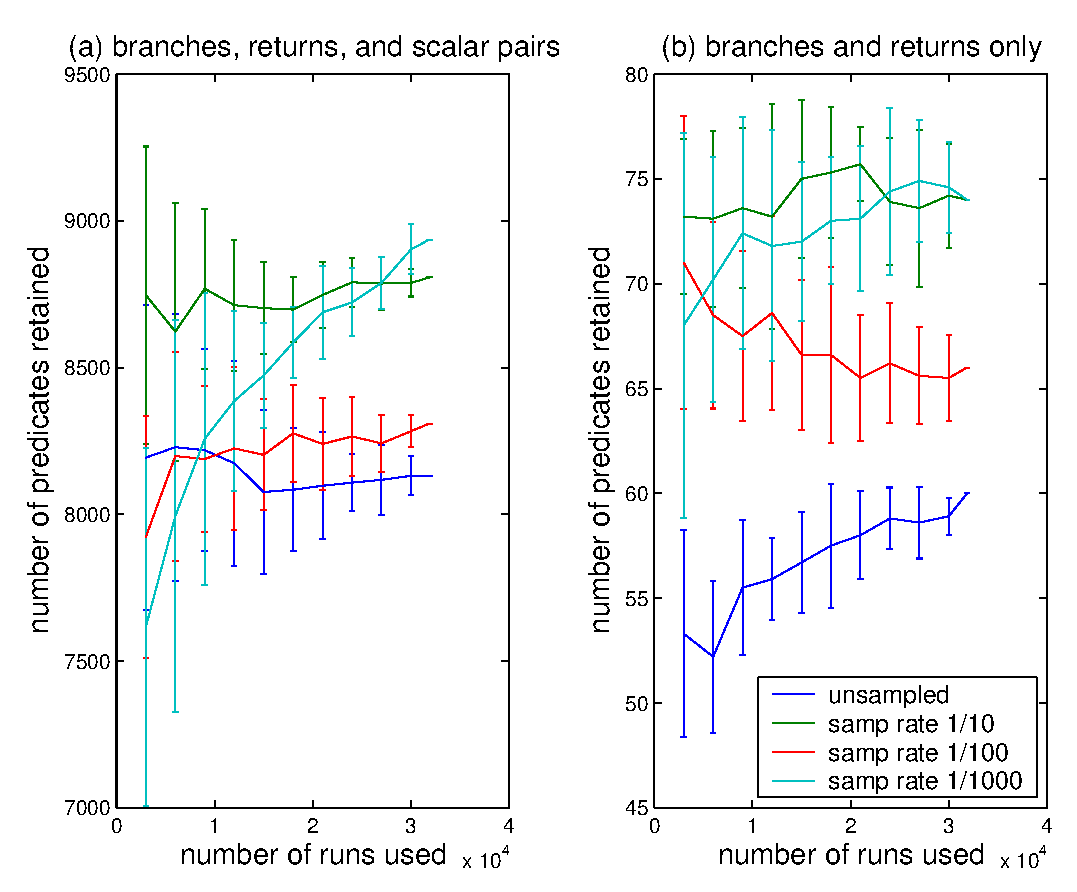
\includegraphics[height=1.5in,width=\columnwidth]{predkept1}
  \caption{The effect of sampling and data size on the number of
  predicates selected.}
  \label{fig-predkept}
\end{figure}

As is apparent from the graph, there is much larger variation in the
number of selected predicates when we use fewer trial runs.
%Using $3000$ trials, at the minimum we
%retain $7429$ predicates using unsampled data, $7654$ when sampling
%rate is $\nicefrac{1}{10}$, $7347$ at $\nicefrac{1}{100}$, and $6750$
%at $\nicefrac{1}{1000}$;
As we incorporate more successful and failed \moss\ runs, the variance
decrease for all sampling rates, but the mean behaves
somewhat differently.  When the data is not sampled, the average
number of selected predicates stay around $8100$ for all data sizes.
Sampling adds noise to this procedure and tend to increase our set of
selected predicates (except when sampling is very sparse or we are
using very few trial runs).

At the relatively high sampling rate of
\nicefrac{1}{10}, there are still enough samples taken at most
instrumentation sites, and there's a net increase in the number of
selected predicates.  Once the sampling rate increases to
\nicefrac{1}{100} and above, however, the sparsifying effect of
sampling sets in; fewer samples are taken overall on fewer predicates,
and as a result, fewer predicates have a nonzero \increase score.
Incorporating more runs tend to alleviate the situation; at above
$10000$ runs, roughly the same number of predicates are retained for
the \nicefrac{1}{100} sampled data as the unsampled data.  The very
sparse sampling rate of \nicefrac{1}{1000}, on the other hand,
causes much more change in the final result.  A lot more predicates
are eliminated when using fewer trials, and a lot more predicates are
retained using more trials.

Most of the volatility in the results come from the scalar-pairs
predicates.  Figure~\ref{fig-predkept}(b) shows the same graph for
only the branch and return predicates.  Here, across all datasizes,
the number of selected predicates remains roughly constant at each
sampling rate.  The unsampled data is still able to select the fewest
number of predicates, with \nicefrac{1}{100} sampled data following
close behind.  The \nicefrac{1}{1000} sampled data still produces a
net increase in the number of selected predicates.

%% LocalWords:  downsampling lang downsampled
